\documentclass[11pt, aspectratio=169, xcolor=table]{beamer}
\usepackage[utf8]{inputenc}
\usepackage[T1]{fontenc}
\usepackage{graphicx}
\usepackage{hyperref}
\usepackage{lmodern}
\usepackage[spanish]{babel}
\usepackage{pdfrender}
\usepackage{xcolor}
\usepackage{ragged2e}
\usepackage[version=4]{mhchem}
\usepackage{siunitx}
\usepackage{amsmath}
\renewcommand{\raggedright}{\justifying}
\usepackage{smartdiagram}
\usetheme{Berlin}

% Start every section with a frame
\AtBeginSection[]
{
  \begin{frame}
    \frametitle{Table of Contents}
    \tableofcontents[currentsection]
  \end{frame}
}


\author{Prof. Daniel Muñoz \\
	\texttt{daniel.munoz3@mail.udp}.cl
}
\title{Química Unidad 4}
\subtitle{Química del agua. Desde la industria hasta el medioambiente}

\begin{document}

\maketitle

\section{Unidades de concentración física (porcentajes p/p, p/v y v/v). Cálculos en disoluciones con concentraciones molares.}

\begin{frame}[allowdisplaybreaks]
	\frametitle{Introducción}
	\begin{columns}
		\begin{column}{.5\textwidth}
			\begin{itemize}[<+->]
				\item ¿Qué es una disolución? $\rightarrow$ Mezcla homogénea de soluto y disolvente.
				\item Componentes: soluto (en menor cantidad) y disolvente (en mayor cantidad).
				\item Ejemplos cotidianos: suero fisiológico, jugos, soluciones limpiadoras.
				\item Importancia de medir ``cuánto'' soluto hay en una disolución.
				\item Las distintas formas de expresar concentración responden a diferentes contextos: industria, laboratorio, medioambiente.
			\end{itemize}
		\end{column}

		\begin{column}{.5\textwidth}
			\begin{figure}[ht]
				\centering
				\includegraphics[width=\textwidth]{../img/mezcla.png}
				\caption{\label{fig:label} Mezcla a nivel microscópico}
			\end{figure}

		\end{column}
	\end{columns}
\end{frame}

\begin{frame}[allowdisplaybreaks]
	\frametitle{Unidades de Concentración Físicas}
	\begin{columns}
		\begin{column}{.5\textwidth}
			\textbf{Definiciones:}
			\begin{itemize}[<+->]
				\small
				\item \% m/m (p/p): (masa soluto / masa disolución) $\times$  100
				\item Ej.: 10 g NaCl en 90 g \ce{H2O} $\rightarrow$ disolución 10 \% p/p
				\item \% m/v (p/v): (masa soluto / volumen disolución) $\times$ 100
				\item Ej.: 5 g glucosa en 100 mL solución $\rightarrow$ 5 \% p/v
				\item \% v/v: (volumen soluto / volumen disolución) $\times$ 100
				\item Ej.: 40 mL etanol en 100 mL disolución $\rightarrow$ 40 \% v/v
			\end{itemize}
		\end{column}

		\begin{column}{.5\textwidth}
			\begin{block}{Usos}
				\begin{itemize}[<+->]
					\item p/p: común en industria alimentaria y farmacéutica.
					\item p/v: común en soluciones de laboratorio.
					\item v/v: común en soluciones líquidas miscibles (alcohol, perfumes).
				\end{itemize}
			\end{block}
		\end{column}
	\end{columns}
\end{frame}

\begin{frame}[allowdisplaybreaks]
	\frametitle{Ejemplo}
	\begin{columns}
		\begin{column}{.5\textwidth}
			\begin{exampleblock}{Problema}
				¿Cuál es el \% p/v de una disolución con 5,0 g de NaCl en 250 mL?
			\end{exampleblock}
		\end{column}

		\begin{column}{.5\textwidth}

		\end{column}
	\end{columns}
\end{frame}

\begin{frame}[allowdisplaybreaks]
	\frametitle{Concentración Molar}
	\begin{columns}
		\begin{column}{.5\textwidth}
			\textbf{Definición:}
			\begin{itemize}[<+->]
				\item Molaridad (M) = moles de soluto / litros de disolución.
				\item Pasos clave:
				      \begin{itemize}[<+->]
					      \item Calcular moles: n = masa / peso molecular (PM)
					      \item Convertir volumen a litros
					      \item Aplicar fórmula
				      \end{itemize}
			\end{itemize}
		\end{column}

		\begin{column}{.5\textwidth}
			\begin{block}{Importancia}
				\begin{itemize}[<+->]
					\item Base para cálculos estequiométricos y preparación precisa de soluciones.
					\item Permite relacionar directamente masa $\leftrightarrow$ volumen $\leftrightarrow$ cantidad de sustancia.
					\item Unidades: \unit{mol/L} o \unit{\mol\per\litre}
				\end{itemize}
			\end{block}
		\end{column}
	\end{columns}
\end{frame}

\begin{frame}[allowdisplaybreaks]
	\frametitle{Ejemplo 2}
	\begin{columns}
		\begin{column}{.5\textwidth}
			\begin{exampleblock}{Problema}
				Se tienen 100 mL de disolución con 0,56 g de KOH. Determine la concentración molar de la disolución
			\end{exampleblock}

		\end{column}

		\begin{column}{.5\textwidth}

		\end{column}
	\end{columns}
\end{frame}

\begin{frame}[allowdisplaybreaks]
	\frametitle{Ejemplo 3}
	\begin{columns}
		\begin{column}{.5\textwidth}
			\begin{exampleblock}{Problema}
				Determine la concentración molar de una solución de 100 mL de disolución con 0,740 g de \ce{Ca(OH)2}
			\end{exampleblock}

		\end{column}

		\begin{column}{.5\textwidth}

		\end{column}
	\end{columns}

\end{frame}

\section{Definición, Expresión e interpretación de la constante de equilibrio en reacciones ácido base}

\begin{frame}[allowdisplaybreaks]
	\frametitle{Introducción al equilibrio}
	\begin{columns}
		\begin{column}{.5\textwidth}
			\begin{itemize}[<+->]
				\item Un equilibrio químico ocurre cuando la velocidad de la reacción directa es igual a la inversa.
				\item Las concentraciones de reactantes y productos se mantienen constantes en el tiempo.
				\item No implica que reactantes y productos estén en igual cantidad.
				\item Ejemplo cotidiano: Corrosión: Lo que se oxida puede recuperarse: \ce{4Fe + 3O2 -> 2Fe2O3}
			\end{itemize}
		\end{column}

		\begin{column}{.5\textwidth}
			\begin{figure}[ht]
				\centering
				\includegraphics[width=0.6\textwidth]{../img/equilibrio1.jpeg}
				\caption{Existen productos que nos permiten eliminar el óxido.}
			\end{figure}

		\end{column}
	\end{columns}
\end{frame}

\begin{frame}[allowdisplaybreaks]
	\frametitle{Constante de equilibrio}
	\begin{columns}
		\begin{column}{.5\textwidth}
			\begin{itemize}[<+->]
				\small
				\item En una reacción en equilibrio la \textit{velocidad} a la que ocurre:
				      \begin{itemize}[<+->]
					      \small
					      \item la reacción directa:  \ce{2H+(ac) + CO3^2-(ac) -> H2CO3(ac)} es igual a
					      \item la reacción inversa: \ce{H2CO3(ac) -> 2H+(ac) + CO3^2-(ac)} y por tanto
					      \item lo escribimos \ce{2H+(ac) + CO3^2-(ac) <=> H2CO3(ac)}
				      \end{itemize}
				\item El \textit{estado de equilibrio} se cuantifica de la siguiente forma para la reacción ejemplo:
				\item $\frac{[\ce{H2CO3}]}{[\ce{H+}]^{2}[\ce{CO3^2-}]^{2}}$
			\end{itemize}
		\end{column}

		\begin{column}{.5\textwidth}
			\begin{figure}[ht]
				\centering
				\includegraphics[width=.6\textwidth]{../img/vel-eq.png}
				\caption{\label{fig:label} Después de un tiempo de iniciada la reacción las velocidades directa e inversa se igualan}
			\end{figure}

		\end{column}
	\end{columns}
\end{frame}

\begin{frame}[allowdisplaybreaks]
	\frametitle{Constante de equilibrio II}
	\begin{columns}
		\begin{column}{.5\textwidth}
			\begin{itemize}[<+->]
				\item Solo se incluyen las especies en estado acuoso o gaseoso (nunca líquidos puros como el agua).
				\item El valor de K indica hacia qué lado se favorece el equilibrio:
				      \begin{itemize}
					      \item K >> 1 $\rightarrow$ \textit{equilibrio está desplazado} a los productos
					      \item K << 1 $\rightarrow$ \textit{equilibrio está desplazado} a los reactantes
				      \end{itemize}
			\end{itemize}
		\end{column}
		\begin{column}{.5\textwidth}
			\begin{figure}[ht]
				\centering
				\includegraphics[width=\textwidth]{../img/interpretacion-cte.png}
				\caption{\label{fig:label} Interpretación de la constante}
			\end{figure}
		\end{column}
	\end{columns}
\end{frame}

\begin{frame}[allowdisplaybreaks]
	\frametitle{Jacobus Van ’t Hoff}
	\begin{columns}
		\begin{column}{.5\textwidth}
			\begin{itemize}[<+->]
				\item Químico neerlandés 1852 - 1911.
				\item Estudió Química en la Universidad Bonn, Paris, dónde coincidió con \textit{Kekulé} como su profesor.
				\item Van ’t Hoff desarrolló la teoría del equilibrio químico y su relación con la energía. Entre muchas otras más.
				\item Estableció cómo las concentraciones se relacionan con el equilibrio mediante ecuaciones cuantitativas.
				\item Premio Nobel de Química 1901.
			\end{itemize}
		\end{column}

		\begin{column}{.5\textwidth}
			\begin{figure}[ht]
				\centering
				\includegraphics[height=0.6\textheight]{../img/vanthoff.png}
				\caption{\label{fig:label} Foto aprox. 1900}
			\end{figure}

		\end{column}
	\end{columns}
\end{frame}

\begin{frame}[allowdisplaybreaks]
	\frametitle{Ejemplo}
	\begin{columns}
		\begin{column}{.5\textwidth}
			\begin{exampleblock}{Acidificación de los océanos}
				Exprese la constante de equilibrio de la reacción:
				\ce{CO2(g) + H2O(l) <=> H2CO3}
			\end{exampleblock}

		\end{column}

		\begin{column}{.5\textwidth}

		\end{column}
	\end{columns}
\end{frame}

\section{Predicción del desplazamiento de un equilibrio ácido base en función de las concentraciones de los reactantes o productos}

\begin{frame}[allowdisplaybreaks]
	\frametitle{Predicción del desplazamiento del equilibrio}
	\begin{columns}
		\begin{column}{.5\textwidth}
			\begin{itemize}[<+->]
				\item El equilibrio se puede alterar cambiando:
				      \begin{itemize}[<+->]
					      \item [Reactantes]: desplazamiento hacia productos.
					      \item [Productos]: desplazamiento hacia reactantes.
					      \item Temperatura o presión.
				      \end{itemize}
				\item Principio de Le Châtelier: el sistema tiende a oponerse al cambio impuesto.
			\end{itemize}
		\end{column}

		\begin{column}{.5\textwidth}
			\begin{itemize}[<+->]
				\item $\uparrow P$ como respuesta la rx. : \ce{R <<=> P}
				\item $\uparrow R$ como respuesta la rx. : \ce{R <=>> P}
			\end{itemize}
		\end{column}
	\end{columns}
\end{frame}

\begin{frame}[allowdisplaybreaks]
	\frametitle{Ejemplo. Desplazamiento por aumento de concentración}
	\begin{exampleblock}{Determine hacia dónde se desplaza el equilibrio}
		Sea la reacción: \ce{NH3(ac) + H2O(l) <=> NH4+(ac) + OH-(ac)} responda para:
		\begin{enumerate}
			\item Agregamos \ce{NH3}
			\item Agregamos \ce{NH4+}
		\end{enumerate}
	\end{exampleblock}
\end{frame}

\begin{frame}[allowdisplaybreaks]
	\frametitle{Ejemplo. Reacción en equilibrio gaseoso}
	\begin{exampleblock}{Responda}
		Sea la reacción \ce{NO2(g) + O2(g) <=> NO(g) + O3(g)}
		\begin{enumerate}
			\item ¿Tipo de equilibrio?
			\item Exprese la K
			\item Si se aumenta [\ce{O2}].
		\end{enumerate}

	\end{exampleblock}
\end{frame}

\section{Definición de pH y cálculo de pH de ácidos y bases fuertes}

\begin{frame}[allowdisplaybreaks]
	\frametitle{¿Qué es un ácido y una base?}
	\begin{columns}
		\begin{column}{.5\textwidth}
			\begin{itemize}[<+->]
				\small
				\item Es conocido en la cultura popular el concepto de ácido, pero ¿Qué es un ácido?
				\item En química existen muchas definiciones de ácidos y bases, la primera y más sencilla de ellas dice:.
				\item \textit{Un ácido sustancia que libera iones \ce{H+} en agua.}
				\item Ejemplo: \ce{HCl(ac) -> H+(ac) + Cl-(ac)}
				\item \textit{Una base sustancia que libera iones \ce{OH-} en agua.}
				\item Ejemplo: \ce{NaOH(s) -> Na+(ac) + OH-(ac)}
			\end{itemize}
		\end{column}

		\begin{column}{.5\textwidth}
			\begin{figure}[ht]
				\centering
				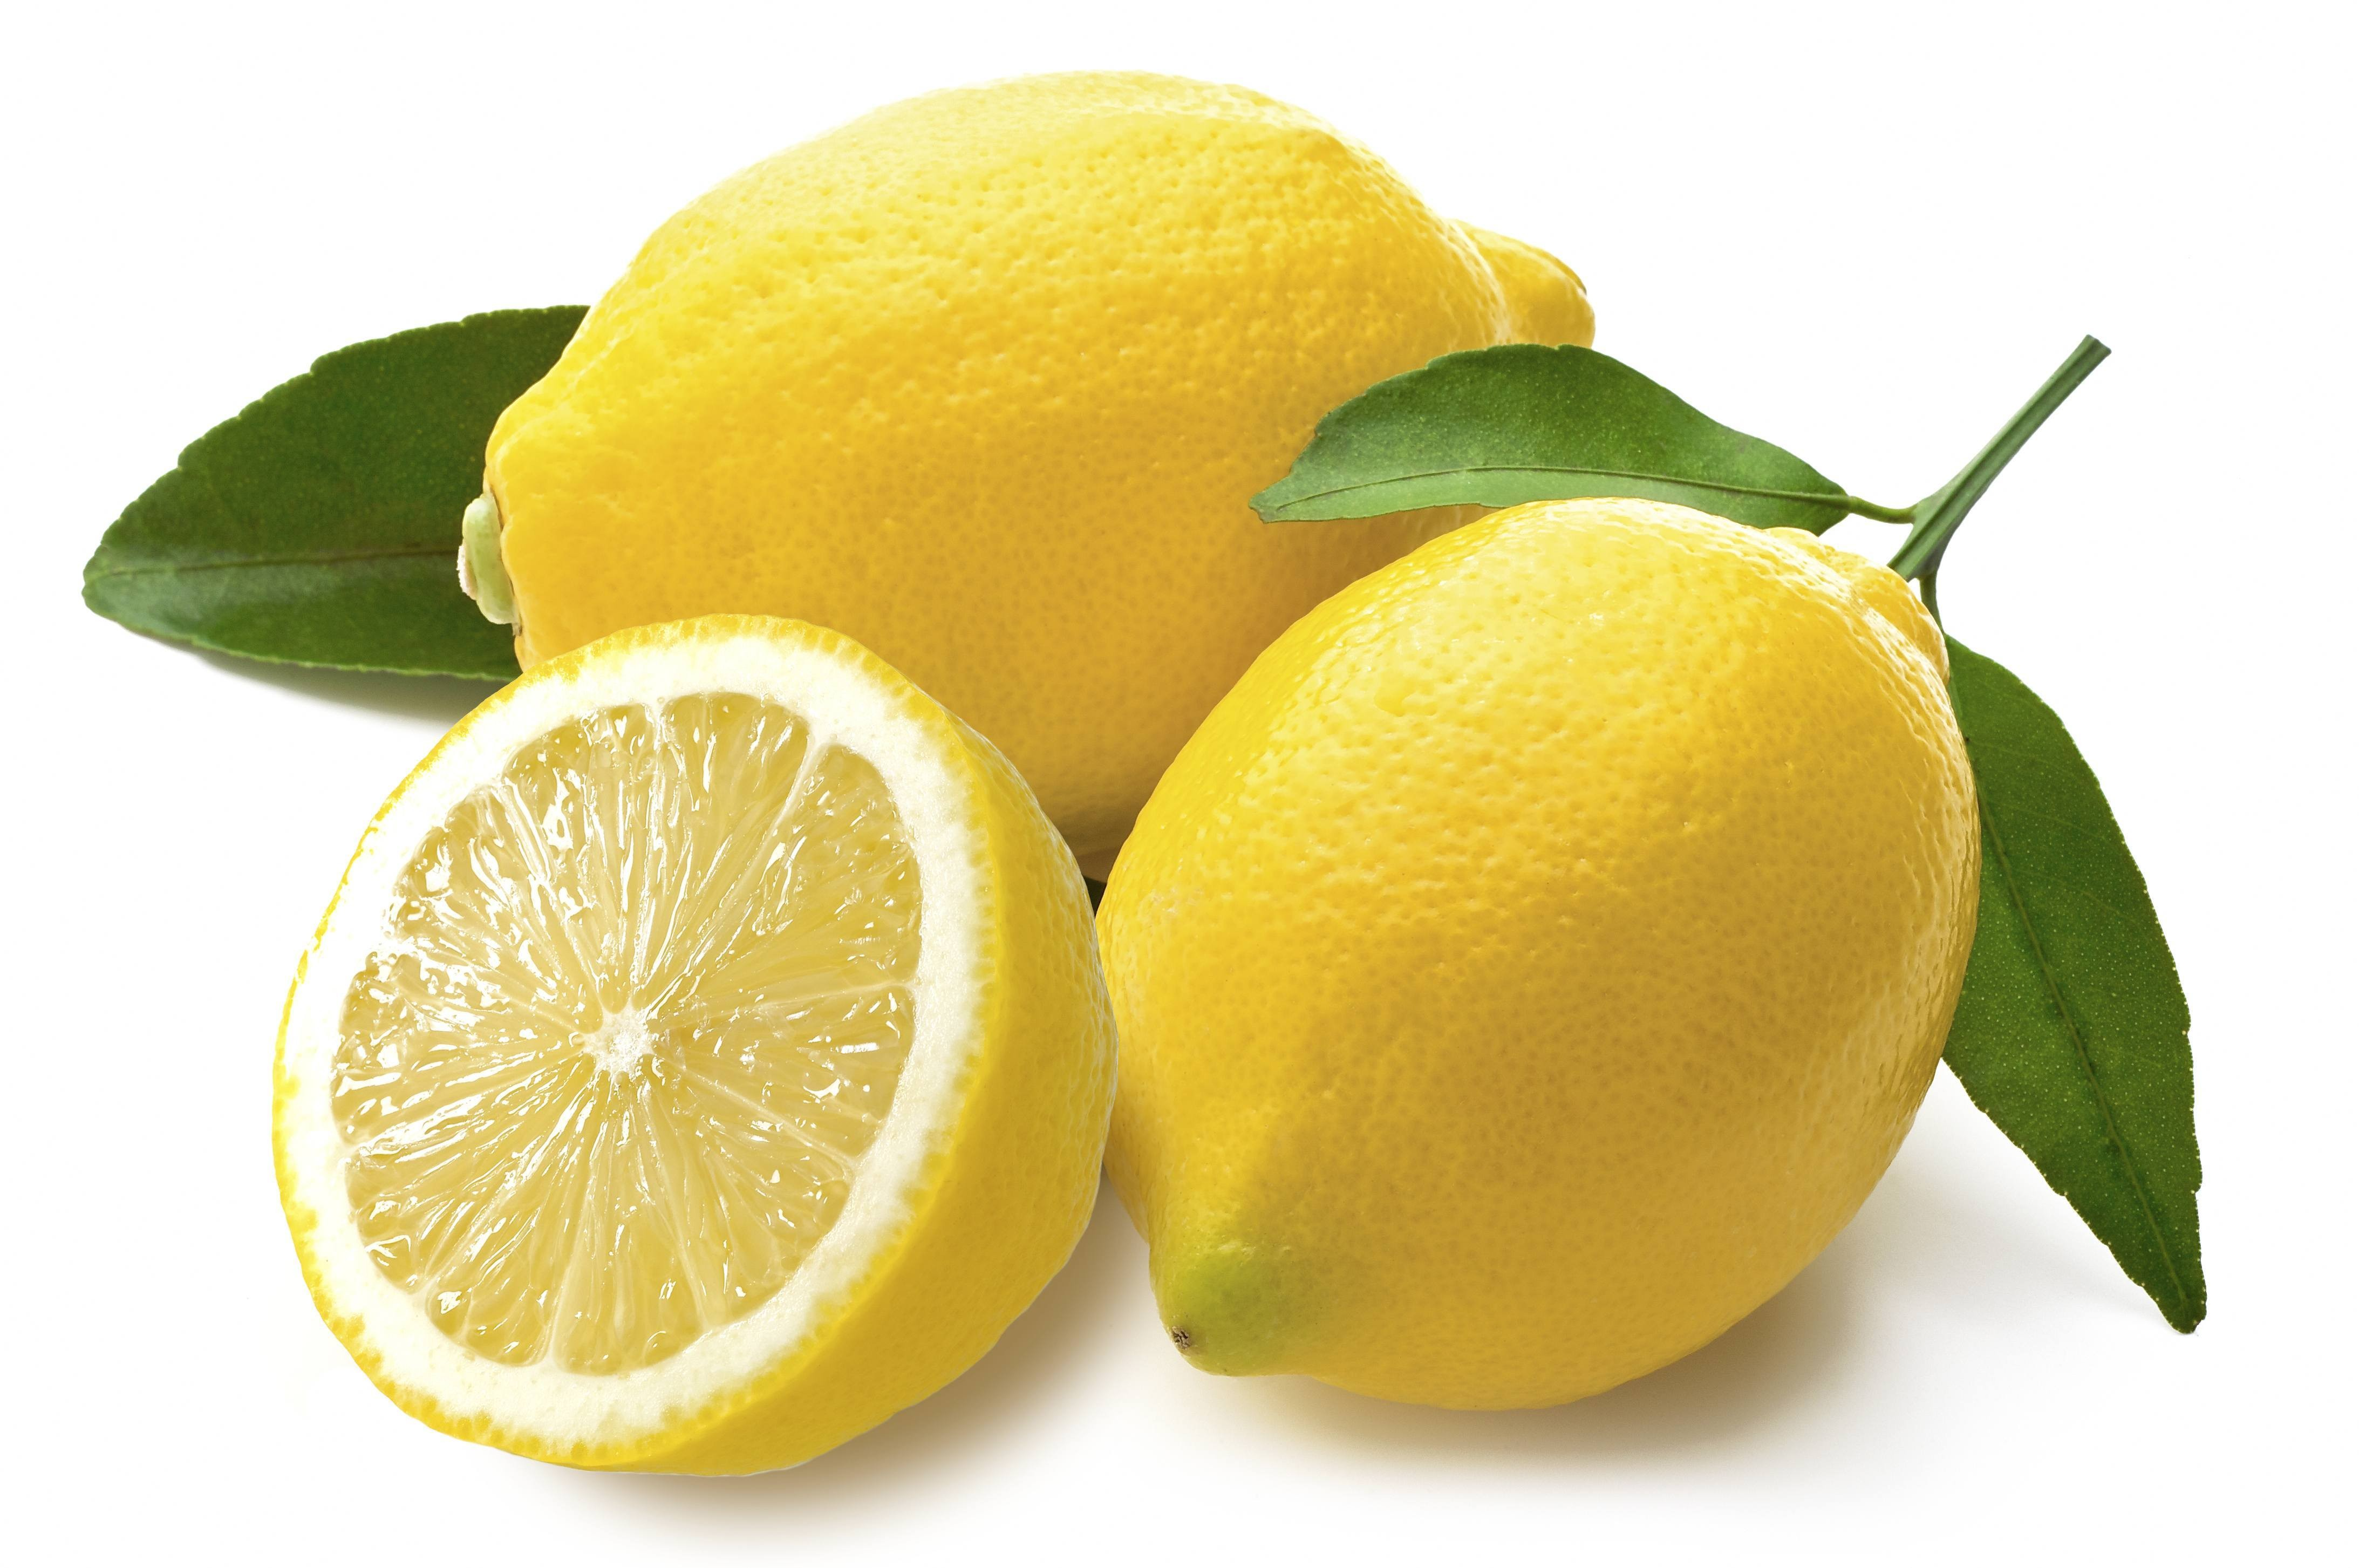
\includegraphics[width=\textwidth]{../img/limon.png}
			\end{figure}

		\end{column}
	\end{columns}
\end{frame}

\begin{frame}[allowdisplaybreaks]
  \frametitle{Svante Arrhenius}
  \begin{columns}
	\begin{column}{.5\textwidth}
	  \begin{itemize}
\item Científico sueco, pionero en la fisicoquímica y galardonado con el Nobel de Química en  1903.
\item Propuso la teoría ácido-base que usamos hasta el día de hoy.
\item Explicó la conductividad eléctrica como resultado de la disociación iónica.
\item Sentó las bases para posteriormente cuantificar la acidez o basicidad de una solución con el pH.
  	  \end{itemize}
	\end{column}

	\begin{column}{.5\textwidth}
\begin{figure}[ht]
  \centering
  \includegraphics[height=.8\textheight]{../img/arrhenius.png}
  \caption{1859 - 1927}
\end{figure}

	\end{column}
  \end{columns}
\end{frame}

\begin{frame}[allowdisplaybreaks]
	\frametitle{Ejemplo. Disociación en agua}
	\begin{columns}
		\begin{column}{.5\textwidth}
			\begin{exampleblock}{Disocie los siguientes ácidos y bases fuertes (disociación completa)}
				\begin{enumerate}
					\item HBr
					\item HI
					\item CsOH
					\item \ce{HNO3}
					\item \ce{H2SO4}
					\item \ce{Ca(OH)2}
				\end{enumerate}
			\end{exampleblock}
		\end{column}
		\begin{column}{.5\textwidth}
		\end{column}
	\end{columns}
\end{frame}

\begin{frame}[allowdisplaybreaks]
	\frametitle{Equilibrio iónico del agua}
	\begin{columns}
		\begin{column}{.5\textwidth}
			\begin{itemize}[<+->]
				\item Si disociamos el \ce{H2O} tenemos: \ce{H2O <=> H+ + OH-}
				\item Entonces: Siempre en una disolución acuosa tendremos iones de \ce{H+} y \ce{OH-}
				\item La cte de equilibrio para el agua (pura) es $K = [\ce{H+}][\ce{OH-}] = \num{1e-14}$
				\item Y en el agua, $[\ce{H+}]=[\ce{OH-}]=\num{1e7}$
			\end{itemize}
		\end{column}

		\begin{column}{.5\textwidth}
			\begin{figure}[ht]
				\centering
				\includegraphics[width=\textwidth]{../img/waterbalance.png}
			\end{figure}

		\end{column}
	\end{columns}
\end{frame}

\begin{frame}[allowdisplaybreaks]
	\frametitle{¿Cómo medir la acidez o basicidad de una solución?}
	\begin{columns}
		\begin{column}{.5\textwidth}
			\begin{itemize}
				\scriptsize
				\item Determinar que tan \textit{ácida} o \textit{básica} es una solución es importante ya que muchos procesos industriales dependen de la cantidad de [\ce{H+}] y [\ce{OH-}].
				\item ¿El problema? Cuando se informan las concentraciones de [\ce{H+}] o [\ce{OH-}] normalmente son valores que rondan 0,000000100 M.
				\item Cifras pequeñas y difíciles de leer. Para superar este problema el científico danés Sørensen (1868-1939) resolvió este problema.
				\item En 1909 mientras trabajaba en la cervecería Carlsen necesitaba comunicar de forma sencilla la acidez y basicidad de la mezcla de cereales.
				\item Y su respuesta fue el pH.
			\end{itemize}
		\end{column}

		\begin{column}{.5\textwidth}
			\begin{figure}[ht]
				\centering
				\includegraphics[height=0.8\textheight]{../img/sorensen.png}
				\caption{Sørensen en su trabajo}
			\end{figure}

		\end{column}
	\end{columns}

\end{frame}

\begin{frame}[allowdisplaybreaks]
	\frametitle{Introducción al concepto de pH: ¿Cómo medir la acidez?}
	\begin{columns}
		\begin{column}{.5\textwidth}
			\begin{itemize}[<+->]
				\item El pH indica la acidez o basicidad de una disolución acuosa.
				\item Se define como: $pH = -\log[\ce{H+}]$
				\item Valores típicos
				      \begin{itemize}[<+->]
					      \item pH < 7 $\rightarrow$ solución ácida.
					      \item pH = 7 $\rightarrow$ neutra.
					      \item pH > 7 $\rightarrow$ básica.
				      \end{itemize}
			\end{itemize}
		\end{column}

		\begin{column}{.5\textwidth}
			\begin{figure}[ht]
				\centering
				\includegraphics[width=\textwidth]{../img/escala-ph.png}
			\end{figure}

		\end{column}
	\end{columns}
\end{frame}

\begin{frame}[allowdisplaybreaks]
	\frametitle{Introducción al concepto de pOH y su relación con el pH}
	\begin{columns}
		\begin{column}{.5\textwidth}
			\begin{itemize}[<+->]
				\item Así como medimos la acidez con el pH, también podemos medir la basicidad con el pOH.
				\item La definición de pOH = $-\log[\ce{OH-}]$
				\item La relación de pH y pOH es inversa, cuando uno aumenta el otro disminuye, ¿Cómo?
			\end{itemize}
		\end{column}

		\begin{column}{.5\textwidth}

		\end{column}
	\end{columns}
\end{frame}

\begin{frame}[allowdisplaybreaks]
	\frametitle{Ejemplo}
	\begin{exampleblock}{Determine el pH y pOH}
		Para una solución:
		\begin{enumerate}
			\item 0,01M de HCl
			\item 0,001M de KOH
			\item 0,005M de \ce{H2SO4} (disociación completa)
			\item 0,005M de \ce{Ca(OH)2} (disociación completa)
		\end{enumerate}

	\end{exampleblock}
\end{frame}

\begin{frame}[allowdisplaybreaks]
	\frametitle{Neutralización Ácido-base}
	\begin{itemize}
		\item ¿Qué sucede cuando un ácido y una base se juntan? se neutralizan
		\item Ejemplo:
		\item \ce{HCl + NaOH -> H2O + NaCl}
		\item Siempre en una neutralización ácido-base, los productos son: un compuesto iónico (sal) y agua.
	\end{itemize}

\end{frame}


\section{Concepto de ácidos y bases débiles. Concepto de buffer.}

\begin{frame}
  \frametitle{Disociación parcial vuelta al concepto de equilibrio: Teoría de Bronsted y Lowry}
  \begin{columns}
    \begin{column}{0.4\textwidth}
      \begin{itemize}
              \footnotesize
        \item Lo que hemos visto hasta ahora son reacciones donde todo los reactantes se transforman en productos
        \item Pero eso no siempre es así, a veces esto es parcial, lo que significa que no todo el reactante se convierte en producto
        \item A esto se le llama equilibrio y cuando las especies son ácidos bases se llamará equilibro ácido base y usaremos dos conceptos:
        \item ``ácido/base fuerte'': Aquella que se disocia \textbf{totalmente} en agua.
        \item ``ácido/base débil'': Aquella que se disocia \textbf{parcialmente} en agua.
      \end{itemize}
    \end{column}
    \begin{column}{0.6\textwidth}
      \begin{definition}
        \begin{itemize}
          \item[$K_a$] \ce{$\underset{\text{ácido}}{\ce{HX}}$ + H2O <--> H3O+ + $\underset{\text{base conjugada}}{\ce{X-}}$}
          \item[$K_b$] \ce{$\underset{\text{base}}{\ce{CaCO3}}$ + H2O <--> CaO + $\underset{\text{ácido conjugado}}{\ce{H2CO3}}$}
          \item \textbf{ácido conjugado}: producto de la disociación de un ácido al ceder protón(es).
          \item \textbf{base conjugada}: producto de la disociación de una base al capturar protón(es).
        \end{itemize}
      \end{definition}
    \end{column}
  \end{columns}
\end{frame}

\begin{frame}
  \frametitle{Concepto de buffer: Solución amortiguadora}
  \begin{columns}
    \begin{column}{0.5\textwidth}
      \begin{itemize}[<+->]
        \item Si tenemos una solución de un ácido y su base conjugada, tendremos lo que se llama una ``solución buffer''.
        \item La gracia de esta solución es que permite mantener el pH amortiguando cambios por agentes externos.
        \item Un ejemplo biológico es nuestra sangra, para que el organismo se mantenga sano el pH de la sangre debe estar entre 7.35 y 7.45.
        \item Entonces, ¿porque no nos enfermamos cuando comémos un limón (pH = 3)?
      \end{itemize}
    \end{column}
    \begin{column}{0.5\textwidth}
      Respuesta:
      \begin{itemize}[<+->]
        \footnotesize
        \item La sangre permite el intercambio de gases en el organismo, pensemos en uno de ellos: \ce{CO2} y su contenido es agua entonces:
        \item \ce{CO2 + H2O -> H2CO3 <--> H+ + HCO3-}
        \item Entonces en nuestra sangre tenemos \ce{H2CO3} y \ce{HCO3-}
        \item Cuando un \ce{H+} entra a nuestra sangre elevando el pH, pasa lo siguiente: \ce{HCO3- + H+ -> H2CO3} impidiendo que H+ actué.
        \item Por otra parte si un \ce{OH-} entra: \ce{H2CO3 + OH- -> HCO3- + H2O} impidiendo que el \ce{OH-} baje el pH.
      \end{itemize}
    \end{column}
  \end{columns}
\end{frame}

\section{Explicar la dureza del agua utilizando KPS.}

\begin{frame}
  \frametitle{Tipos de disolución}
    \begin{itemize}
            \footnotesize
      \item \textbf{Solución saturada}: Contiene el máximo de soluto que se puede disolver.
      \item \textbf{Solución insaturada}: Contiene menos del máximo de soluto que se puede disolver.
      \item \textbf{Solución sobresaturada}: Contiene más del máximo de soluto que se puede disolver (inestable).
      \item \textbf{Forma con precipitado}: Solución saturada que contiene un exceso de soluto no disuelto (precipitado).
    \end{itemize}
    \begin{center}
      \includegraphics[width=0.6\textwidth]{../img/tipossolucion.png}    
    \end{center}
\end{frame}


\begin{frame}
  \frametitle{Solubilidad \cite{Chang2011}}
      \begin{definition}
       \textbf{Solubilidad}: Cantidad de soluto máxima que se puede disolver en un solvente a cierta temperatura, tenemos dos formas de medirla:
        \begin{itemize}
          \item \textbf{Solubilidad Molar:} moles de soluto en un litro de una disolución saturada (\unit[per-mode = fraction]{\mole\per\litre})
          \item \textbf{Solubilidad:} gramos de soluto en un litro de una disolución saturada (\unit[per-mode = fraction]{\gram\per\litre})
        \end{itemize}
      \end{definition}
\end{frame}

\begin{frame}
  \frametitle{Equilibro de producto de solubilidad}
  \begin{columns}
    \begin{column}{0.5\textwidth}
      \begin{itemize}
        \item Los compuestos se pueden disolver hasta cierto punto en una cantidad de solvente, agua.
        \item Algunos compuestos pueden disolverse más otros.
        \item En química podemos cuantificar la cantidad de una sal disuelta, supongamos que disolvemos mucho cloruro de plata en agua:
        \item \ce{AgCl(s) <--> Ag+(aq) + Cl-(aq)}
      \end{itemize}
    \end{column}
    \begin{column}{0.5\textwidth}
      \begin{itemize}
        \item Lo que tenemos es un equilibrio entre el precipitado que se disuelve y lo disuelto que precipita, dado que ni sólidos ni líquidos puros van el constante de equilibrio esta constante se escribiría como:
        \item $K_{ps} = [\ce{Ag+}][\ce{Cl-}]$
      \end{itemize}
      \begin{center}
      \includegraphics[width=0.5\textwidth]{../img/kps.jpg}
      \end{center}
    \end{column}
  \end{columns}
\end{frame}

\begin{frame}
  \frametitle{Ejemplo}
  El producto de solubilidad ($K_{ps}$​) del fluoruro de calcio (\ce{CaF2}​) a \qty{25}{\degreeCelsius} es \num{3.9e-11}. Calcula:
  \begin{itemize}
    \item La solubilidad molar (s) del \ce{CaF2} en agua pura.
    \item La solubilidad en gramos por litro (\unit{\gram\per\litre})
  \end{itemize}
  Datos: $MM_{Ca} = \qty{40.08}{\gram\per\mole}$, $MM_{F} = \qty{19,00}{\gram\per\mole}$ 
\end{frame}


\begin{frame}
  \frametitle{Dureza del agua}
  \begin{columns}
    \begin{column}{0.5\textwidth}
      \begin{itemize}
        \item La \textit{dureza} es un concepto que hace referencia a la cantidad de sales disuelta en el agua.
        \item Mientras más \textit{dura} el agua más sales disuelta, mientras más \textit{blanda}, más ``pura''.
      \end{itemize}
    \end{column}
    \begin{column}{0.5\textwidth}
      \begin{definition}
        \begin{center}
          \textit{Blanda} $\leftarrow$ Dureza $\rightarrow$ \textit{Dura}  
        \end{center}
      \end{definition}
    \end{column}
  \end{columns}
\end{frame}

\begin{frame}
  \frametitle{Relación con el KPS y dureza del agua.}
  \begin{columns}
    \begin{column}{0.5\textwidth}
      \begin{itemize}
        \item ¿Cómo podríamos cuantificar la dureza del agua?
        \item Dado que el agua posee diversas sales disueltas, deberíamos tomar una como parámetro.
        \item Dentro de las sales más comunes que presenta el agua es el carbonato de calcio (\ce{CaCO3}) principal responsable del ``sarro'' en las teteras.
        \item La dureza del agua, generalmente, se mide como miligramos de \ca{CaCO3} disueltos en cada litro agua (\unit{\milli\gram\per\litre}).
      \end{itemize}
    \end{column}
    \begin{column}{0.5\textwidth}
      Clasificación del agua según la OMS\footnote{En santiago el valor es de 300 \unit{\milli\gram\per\litre}}:
      \begin{tabular}{|c|c|} \hline
        \ce{CaCO3} (\unit{\milli\gram\per\litre}) & Tipo \\ \hline
        0-60                                                   & Blanda \\
        61-120                                                        & Moderadamente dura \\
        121 - 180                                                        & Dura \\
        > 180                                                        & Muy Dura \\ \hline
      \end{tabular}
    \end{column}
  \end{columns}
\end{frame}

\section{Definición del concepto de equilibrio REDOX}

\begin{frame}[allowdisplaybreaks]
	\frametitle{Reacciones de óxido-reducción}
	\begin{columns}
		\begin{column}{.5\textwidth}
			\begin{itemize}[<+->]
				\small
				\item Las reacciones ácido-base tenían como centro, según Arrhenius, liberación de iones \ce{H+} y \ce{OH-}, existen otro tipo de reacciones que, en lugar de cambiar las características del medio, ácido o básico, las podemos usar para producir electricidad.
				\item Esas reacciones se denominan reacciones de óxido-reducción (REDOX)
				\item Y su principal característica es que se describen como una transferencia de electrones dónde una especie pierde (oxida) y otra gana (reduce)
			\end{itemize}
		\end{column}

		\begin{column}{.5\textwidth}
			\ce{Zn(ac) + Cu^{+2}(ac) -> Zn^{+2}(ac) + Cu(ac)}
		\end{column}
	\end{columns}
\end{frame}


\begin{frame}[allowdisplaybreaks]
  \frametitle{Michael Faraday}
  \begin{columns}
	\begin{column}{.5\textwidth}
	  \begin{itemize}
        \item Químico/Físico Británico, autodidacta.
        \item Estudió junto a Humphry Davy quién hizo grandes aportes al estudio de la electricidad en reacciones químicas.
        \item Con los trabajos que continuó encontró las relaciones entre la cantidad de sustancia y la cantidad de carga eléctrica.
        \item También introdujo los conceptos de reducción, oxidación, cátodo, ánodo, ión, anión, catión.
	  \end{itemize}
	\end{column}

	\begin{column}{.5\textwidth}
\begin{figure}[ht]
  \centering
  \includegraphics[height=0.6\textheight]{../img/faraday.jpg}
  \caption{1791 - 1867}
\end{figure}

	\end{column}
  \end{columns}

\end{frame}

\section{Determinación de los estados de oxidación de las especies químicas}

\begin{frame}[allowdisplaybreaks]
	\frametitle{Estado de oxidación}
	\begin{columns}
		\begin{column}{.5\textwidth}
			\begin{itemize}
				\item Las especies, como bien estudiamos al inicio del curso, pueden perder, ganar o compartir electrones.
				\item El concepto de estado de oxidación, viene a ser una simplificación de lo anterior.
				\item Asume que dentro de una especie química todos los átomos que la componente, ganan (-) o pierden (+) electrones.
				\item A ese número se le conoce como \textit{estado de oxidación}.
			\end{itemize}
		\end{column}

		\begin{column}{.5\textwidth}
			\begin{itemize}
				\item \ce{CH4}
				\item \ce{CO2}
				\item \ce{NaCl}
				\item \ce{H2}
			\end{itemize}
		\end{column}
	\end{columns}

\end{frame}

\begin{frame}[allowdisplaybreaks]
	\frametitle{Reglas para calcular estados de oxidación}
	\begin{enumerate}
		\item Cada elemento de un compuesto químico presenta su EO.
		\item La suma de los EO es la carga de la especie.
		\item El elemento más electronegativo gana y el menos pierde.
		\item El EO en un elemento, ejemplo \ce{H2} es 0
		\item La mayoría de las veces el O tiene valor -2.
		\item Los metales alcalinos tiene valor de +1.
		\item El H tiene valor de +1 a menos que esté con un metal.
	\end{enumerate}
\end{frame}

\begin{frame}[allowdisplaybreaks]
	\frametitle{Ejemplo}
	\begin{columns}
		\begin{column}{.5\textwidth}
			\begin{exampleblock}{Determine los EO de:}
				\begin{itemize}
					\item \ce{CH4}
					\item \ce{NaOH}
					\item \ce{CH3OH}
					\item \ce{H2SO4}
					\item \ce{Na2ClO4}
				\end{itemize}
			\end{exampleblock}
		\end{column}

		\begin{column}{.5\textwidth}

		\end{column}
	\end{columns}
\end{frame}

\begin{frame}[allowdisplaybreaks]
	\frametitle{Ejemplo 2}
	\begin{exampleblock}{Determine los EO en las siguientes reacciones:}
		\begin{enumerate}
			\small
			\item \ce{4Al + 3O2 -> 2Al2O3}
			\item \ce{2SO2 + O2 -> SO3}
			\item \ce{2CuSO4 + 4KI -> 2CuI + I2 + 2K2SO4}
			\item \ce{H2S + Cl2 -> S + 2HCl}
			\item \ce{3PbO + 2NH3 -> N2 + 3H2O + 3Pb}
		\end{enumerate}
	\end{exampleblock}
\end{frame}

\section{Interpretación del pH en ejemplos de procesos ambientales y en sistemas biológicos.}

\begin{frame}
  \frametitle{Lluvia ácida}
  \begin{columns}
    \begin{column}{0.5\textwidth}
      \begin{itemize}
        \item La lluvia tiene un pH $\approx$ 5,6 (ligeramente ácida por el \ce{CO2} atmosférico)
        \item Pero, actualmente las lluvias tienen un pH $\approx$ 5 ¿Por qué?
        \item Presencia de \ce{SO2} y \ce{NO2} dada combustión de combustibles fósiles:
        \item \ce{2SO2 + O2 + H2O -> H2SO4} (ácido sulfúrico)
        \item \ce{4NO2 + 2H2O + O2 -> 4HNO3} (ácido nítrico)
      \end{itemize}
    \end{column}
    \begin{column}{0.5\textwidth}
      \begin{block}{Impactos}
        \begin{itemize}
          \item Afecta la respiración de peces por daño en branquias
          \item Moviliza metales tóxicos del sedimento (\ce{Al^{+3}}, \ce{Pb^{+2}})
          \item Altera reproducción de anfibios
          \item Lixiviación de nutrientes (\ca{Ca^{+2}}, \ce{Mg^{+2}}, \ce{K+})
          \item Liberación de \ce{Al^{+3}} tóxico para raíces.
          \item Muerte de vegetación.
        \end{itemize}
      \end{block}
    \end{column}
  \end{columns}
\end{frame}

\begin{frame}
  \frametitle{Acidificación de los océanos}
  \begin{columns}
    \begin{column}{0.5\textwidth}
      \begin{itemize}
        \item El exceso de \ce{CO2} atmosférico produce acidificación de los océanos.
        \item \ce{CO2 + H2O -> H2CO3} (ácido carbónico)
        \item \ce{H2CO3 -> 2H+ + CO3-2}
      \end{itemize}
    \end{column}
    \begin{column}{0.5\textwidth}
      \begin{alertblock}{Consecuencias}
        \begin{itemize}
          \item Al existir un exceso de \ce{H+} corales y moluscos presentan dificultades para formar sus exoesqueletos, ya que:
          \item \ce{CaCO3 + 2H+ -> H2CO3 + Ca^{+2}} por lo tanto existe una competencia por el ión carbonato (\ce{CO3^{-2}}) entré el exoesqueleto del molusco (\ce{Ca^{+2}}) y el ácido aportado por el \ce{CO2}
        \end{itemize}
      \end{alertblock}
    \end{column}
  \end{columns}
\end{frame}

\begin{frame}
  \frametitle{Actividad biológica en suelos}
  \begin{columns}
    \begin{column}{0.5\textwidth}
      \begin{itemize}
        \item En general la agricultura necesita de suelos con pH $\approx$ 6,0 a 7,5 
        \item Cuando el pH del suelo es bajo, < 5.5
        \item Toxicidad por aluminio
        \item Baja disponibilidad de P, Ca y Mg.
        \item actividad microbiana reducida
        \item Para solucionarlo, adición \ce{CaCO3} al suelo
      \end{itemize}
    \end{column}
    \begin{column}{0.5\textwidth}
      \begin{itemize}
        \item Cuando el pH es alto, > 8.0
        \item Baja disponibilidad de Fe, Mn, Zn
        \item Problemas de absorción de nutrientes
        \item Para solucionarlo, adición de azufre.
      \end{itemize}
    \end{column}
  \end{columns}
\end{frame}

\begin{frame}
  \frametitle{pH y actividad enzimática}
  \begin{columns}
    \begin{column}{0.4\textwidth}
      \begin{itemize}
        \item Las enzimas son proteínas que permiten que ocurran o no ciertas reacciones en los organismos vivos, sin ellas la vida no sería posible
        \item Cada enzima debe tener su pH óptimo, lejos de ese pH la enzima no trabaja.
      \end{itemize}
    \end{column}
    \begin{column}{0.6\textwidth}
      \begin{tabular}{|c|c|c|} \hline
        Enzima & Ubicación & pH óptimo \\ \hline
        Pepsina & Estómago & 2.0 \\
        Tripsina  & Intestino Delgado & 8.0 \\
        Amilasa Salibal & Boca & 6.8 \\ \hline
      \end{tabular}
    \end{column}
  \end{columns}
\end{frame}


\begin{frame}
  \frametitle{Bibliografía}
  \begin{thebibliography}{99}
    \setbeamertemplate{bibliography item}[book]
    \bibitem[Chang, 2011]{Chang2011}
    Chang, Raymond
    \newblock \emph{Fundamentos de Química}
  \end{thebibliography}
\end{frame}
\end{document}
